% Compile with XeLaTeX:
% xelatex CG_Project_Slides_en.tex
\documentclass[aspectratio=169]{beamer}
\usepackage{amsmath,booktabs,graphicx,xcolor}
\usetheme{Madrid}
\definecolor{teal}{RGB}{20,122,131}
\definecolor{coral}{RGB}{219,112,78}
\setbeamercolor{structure}{fg=teal}
\setbeamertemplate{navigation symbols}{}
\setbeamertemplate{footline}[frame number]
\title{Perspective-Correct Texture Mapping in a Software Rasterizer}
\subtitle{UV interpolation and budgeted collaborative filtering}
\author{Computer Graphics Course Project\\Team members: to be added}
\date{2026}
\begin{document}
\begin{frame}\titlepage\end{frame}

\begin{frame}{Affine UVs stretch the checkerboard at 60 degrees}
\begin{columns}[T]
\column{.48\textwidth}\centering\textcolor{coral}{Affine screen-space UV}\\[3pt]
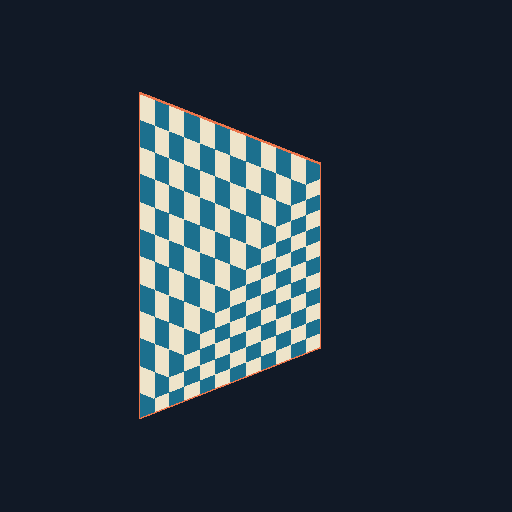
\includegraphics[width=.88\linewidth]{figures/angle_60_affine.png}
\column{.48\textwidth}\centering\textcolor{teal}{Perspective-correct UV}\\[3pt]
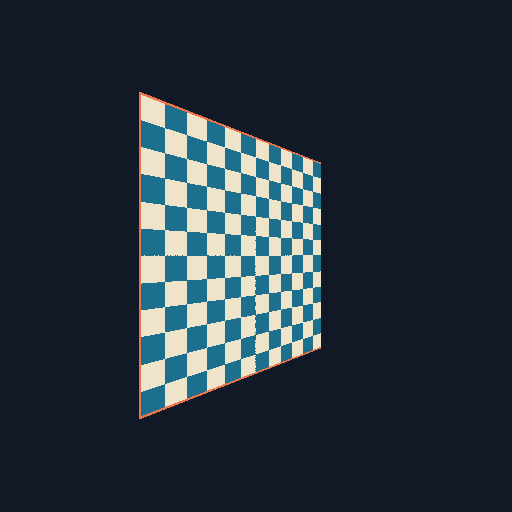
\includegraphics[width=.88\linewidth]{figures/angle_60_perspective.png}
\end{columns}
\vspace{4pt}\centering Same quad, camera, texture, coverage test, and depth buffer. Only the UV interpolation formula changes.
\end{frame}

\begin{frame}{Research question and controlled comparison}
\textcolor{teal}{Research question}
\begin{block}{Question}
How does UV interpolation error grow as a textured plane rotates into perspective?
\end{block}
The camera, quad, generated checkerboard, raster coverage, and depth test stay fixed across both modes.
\vspace{8pt}
\begin{alertblock}{Only one rendering rule changes}
The UV interpolation formula.
\end{alertblock}
\end{frame}

\begin{frame}{The two texture-coordinate formulas}
\begin{columns}[T]
\column{.48\textwidth}\textcolor{coral}{\textbf{Affine interpolation}}
\[
uv=\lambda_0uv_0+\lambda_1uv_1+\lambda_2uv_2
\]
\column{.48\textwidth}\textcolor{teal}{\textbf{Perspective-correct interpolation}}
\[
uv=\frac{\sum_i\lambda_i uv_i/w_i}{\sum_i\lambda_i/w_i}
\]
\end{columns}
\vspace{15pt}
Here $\lambda_i$ are screen-space barycentric coordinates and $w_i$ is the clip-space homogeneous coordinate. In GLSL, \texttt{smooth} uses perspective-correct interpolation, while \texttt{noperspective} is linear in screen space.
\end{frame}

\begin{frame}{CPU rasterizer and experiment settings}
\begin{tabular}{ll}
\textbf{Stage} & \textbf{Implementation}\\\hline
Transform & Model rotation and $52^\circ$ perspective projection\\
Rasterize & Edge functions and barycentric coverage at pixel centers\\
Visibility & Interpolated depth with a software Z-buffer\\
Texture & Generated $256\times256$ checkerboard; nearest-neighbor sampling\\
Sweep & Six angles from $0^\circ$ to $70^\circ$; $512\times512$ output
\end{tabular}
\end{frame}

\begin{frame}{UV error rises as perspective depth variation grows}
\centering
\begin{tabular}{c|rrrrrr}
Angle & 0 & 15 & 30 & 45 & 60 & 70\\\hline
Mean UV error & 0.00 & 8.14 & 15.76 & 22.18 & 27.34 & 29.54\\
P95 UV error & 0.00 & 13.47 & 26.13 & 37.14 & 45.76 & 49.80
\end{tabular}
\vspace{12pt}

\textcolor{teal}{Coordinate distance is measured against the perspective-correct UV value at each shared covered pixel.}
\end{frame}

\begin{frame}{UV error grows; RGB error follows texel edges}
\begin{table}\centering\small
\begin{tabular}{r|rrr}
Angle & Mean UV (texels) & P95 UV (texels) & RGB MAE\\\hline
0 & 0.00 & 0.00 & 0.02\\
15 & 8.14 & 13.47 & 46.43\\
30 & 15.76 & 26.13 & 58.63\\
45 & 22.18 & 37.14 & 57.02\\
60 & 27.34 & 45.76 & 59.83\\
70 & 29.54 & 49.80 & 60.68
\end{tabular}\end{table}
\begin{block}{Observation}
At $70^\circ$, mean UV error reaches 29.54 texture pixels and P95 reaches 49.80. RGB MAE is not perfectly monotonic because nearest-neighbor sampling changes abruptly at texel boundaries.
\end{block}
\end{frame}

\begin{frame}{A second filter, with one evaluation per pixel}
UV interpolation chooses the sample location. Reconstruction chooses how many texels are read there.
\vspace{8pt}
\begin{columns}[T]
\column{.48\textwidth}
\textcolor{coral}{\textbf{Exact Catmull--Rom}}
\begin{itemize}
\item $4\times4$ support, 16 texels
\item Reference filter
\end{itemize}
\column{.48\textwidth}
\textcolor{teal}{\textbf{Mask Sampling + C+}}
\begin{itemize}
\item $8\times4$ tiles, at most one evaluation per covered pixel
\item Exact when the shared footprint fits; otherwise the HPG 2025 fallback
\end{itemize}
\end{columns}
\vspace{8pt}
The two-tap baseline draws the positive and negative Catmull--Rom lobes separately and always costs two evaluations. Akenine-M\"oller et al., Collaborative Texture Filtering, HPG 2025.
\end{frame}

\begin{frame}{Magnification decides whether the budget is exact}
\centering
\small
\begin{tabular}{rrrrrr}
\toprule
Size & Angle & Mag. & Full exact & C+ (dB) & Two-tap (dB)\\\midrule
$32^2$ & $0^\circ$ & 10.52 & 100\% & 58.22 & 14.32\\
$32^2$ & $70^\circ$ & 6.63 & 90.9\% & 57.31 & 14.35\\
$128^2$ & $0^\circ$ & 2.63 & 19.9\% & 57.28 & 23.31\\
$512^2$ & $70^\circ$ & 0.41 & 0\% & 33.54 & 32.07\\
\bottomrule
\end{tabular}
\vspace{8pt}

\normalsize At $32^2$ and $0^\circ$, C+ uses \textbf{0.61} evaluations per pixel against 16 for the cubic. PSNR is the mean of three textures and four seeds, measured against the 16-tap filter.
\end{frame}

\begin{frame}{The same crop at high and low magnification}
\centering
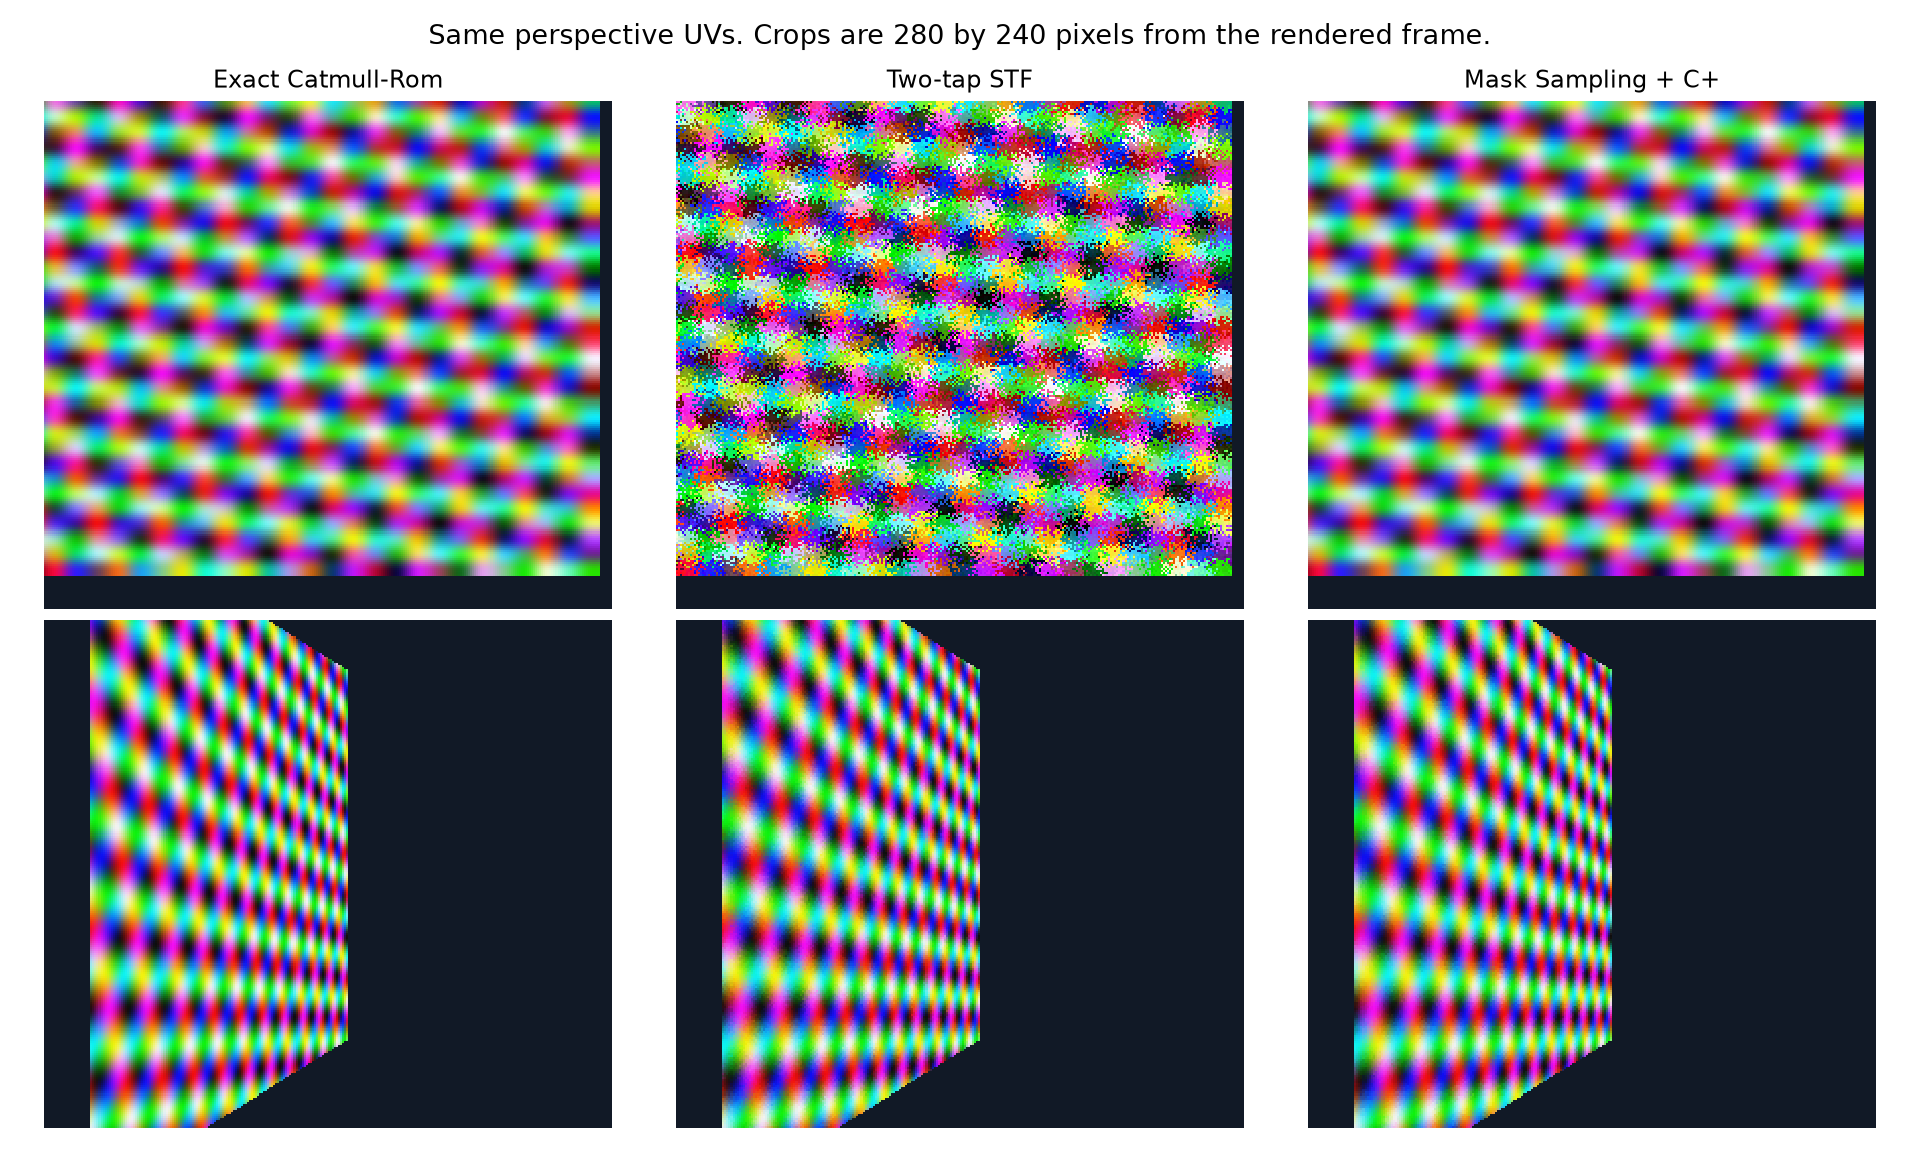
\includegraphics[width=\textwidth,height=.72\textheight,keepaspectratio]{figures/comparison_sota.png}
\vspace{4pt}

{\small Top, $32^2$ at $0^\circ$: collaborative filtering matches Catmull--Rom. Bottom, $512^2$ at $70^\circ$: the footprint no longer fits, and the methods converge.}
\end{frame}

\begin{frame}{Conclusion and scope}
\begin{block}{Conclusion}
Perspective correction removes geometric UV error. Under magnification, Mask Sampling reproduces Catmull--Rom inside a one-evaluation budget; under minification that exactness stops.
\end{block}
\begin{itemize}
\item One planar quad and synthetic textures.
\item CPU tile model: logical evaluations, not GPU timing.
\item No mipmaps, denoiser, neural decoder, or wave intrinsics.
\end{itemize}
\vfill\centering Thank you
\end{frame}
\end{document}
